Kontekst Sprzedaży stanowi nadrzędny, główny obszar działalności biznesowej systemu. Zarządza on bezpośrednimi relacjami z klientem, kalkulacją ofertową oraz cyklem życia kontraktu sprzedażowego.

\subsubsection{Kanwa Kontekstu Sprzedaży}

\begin{figure}[H]
    \centering
    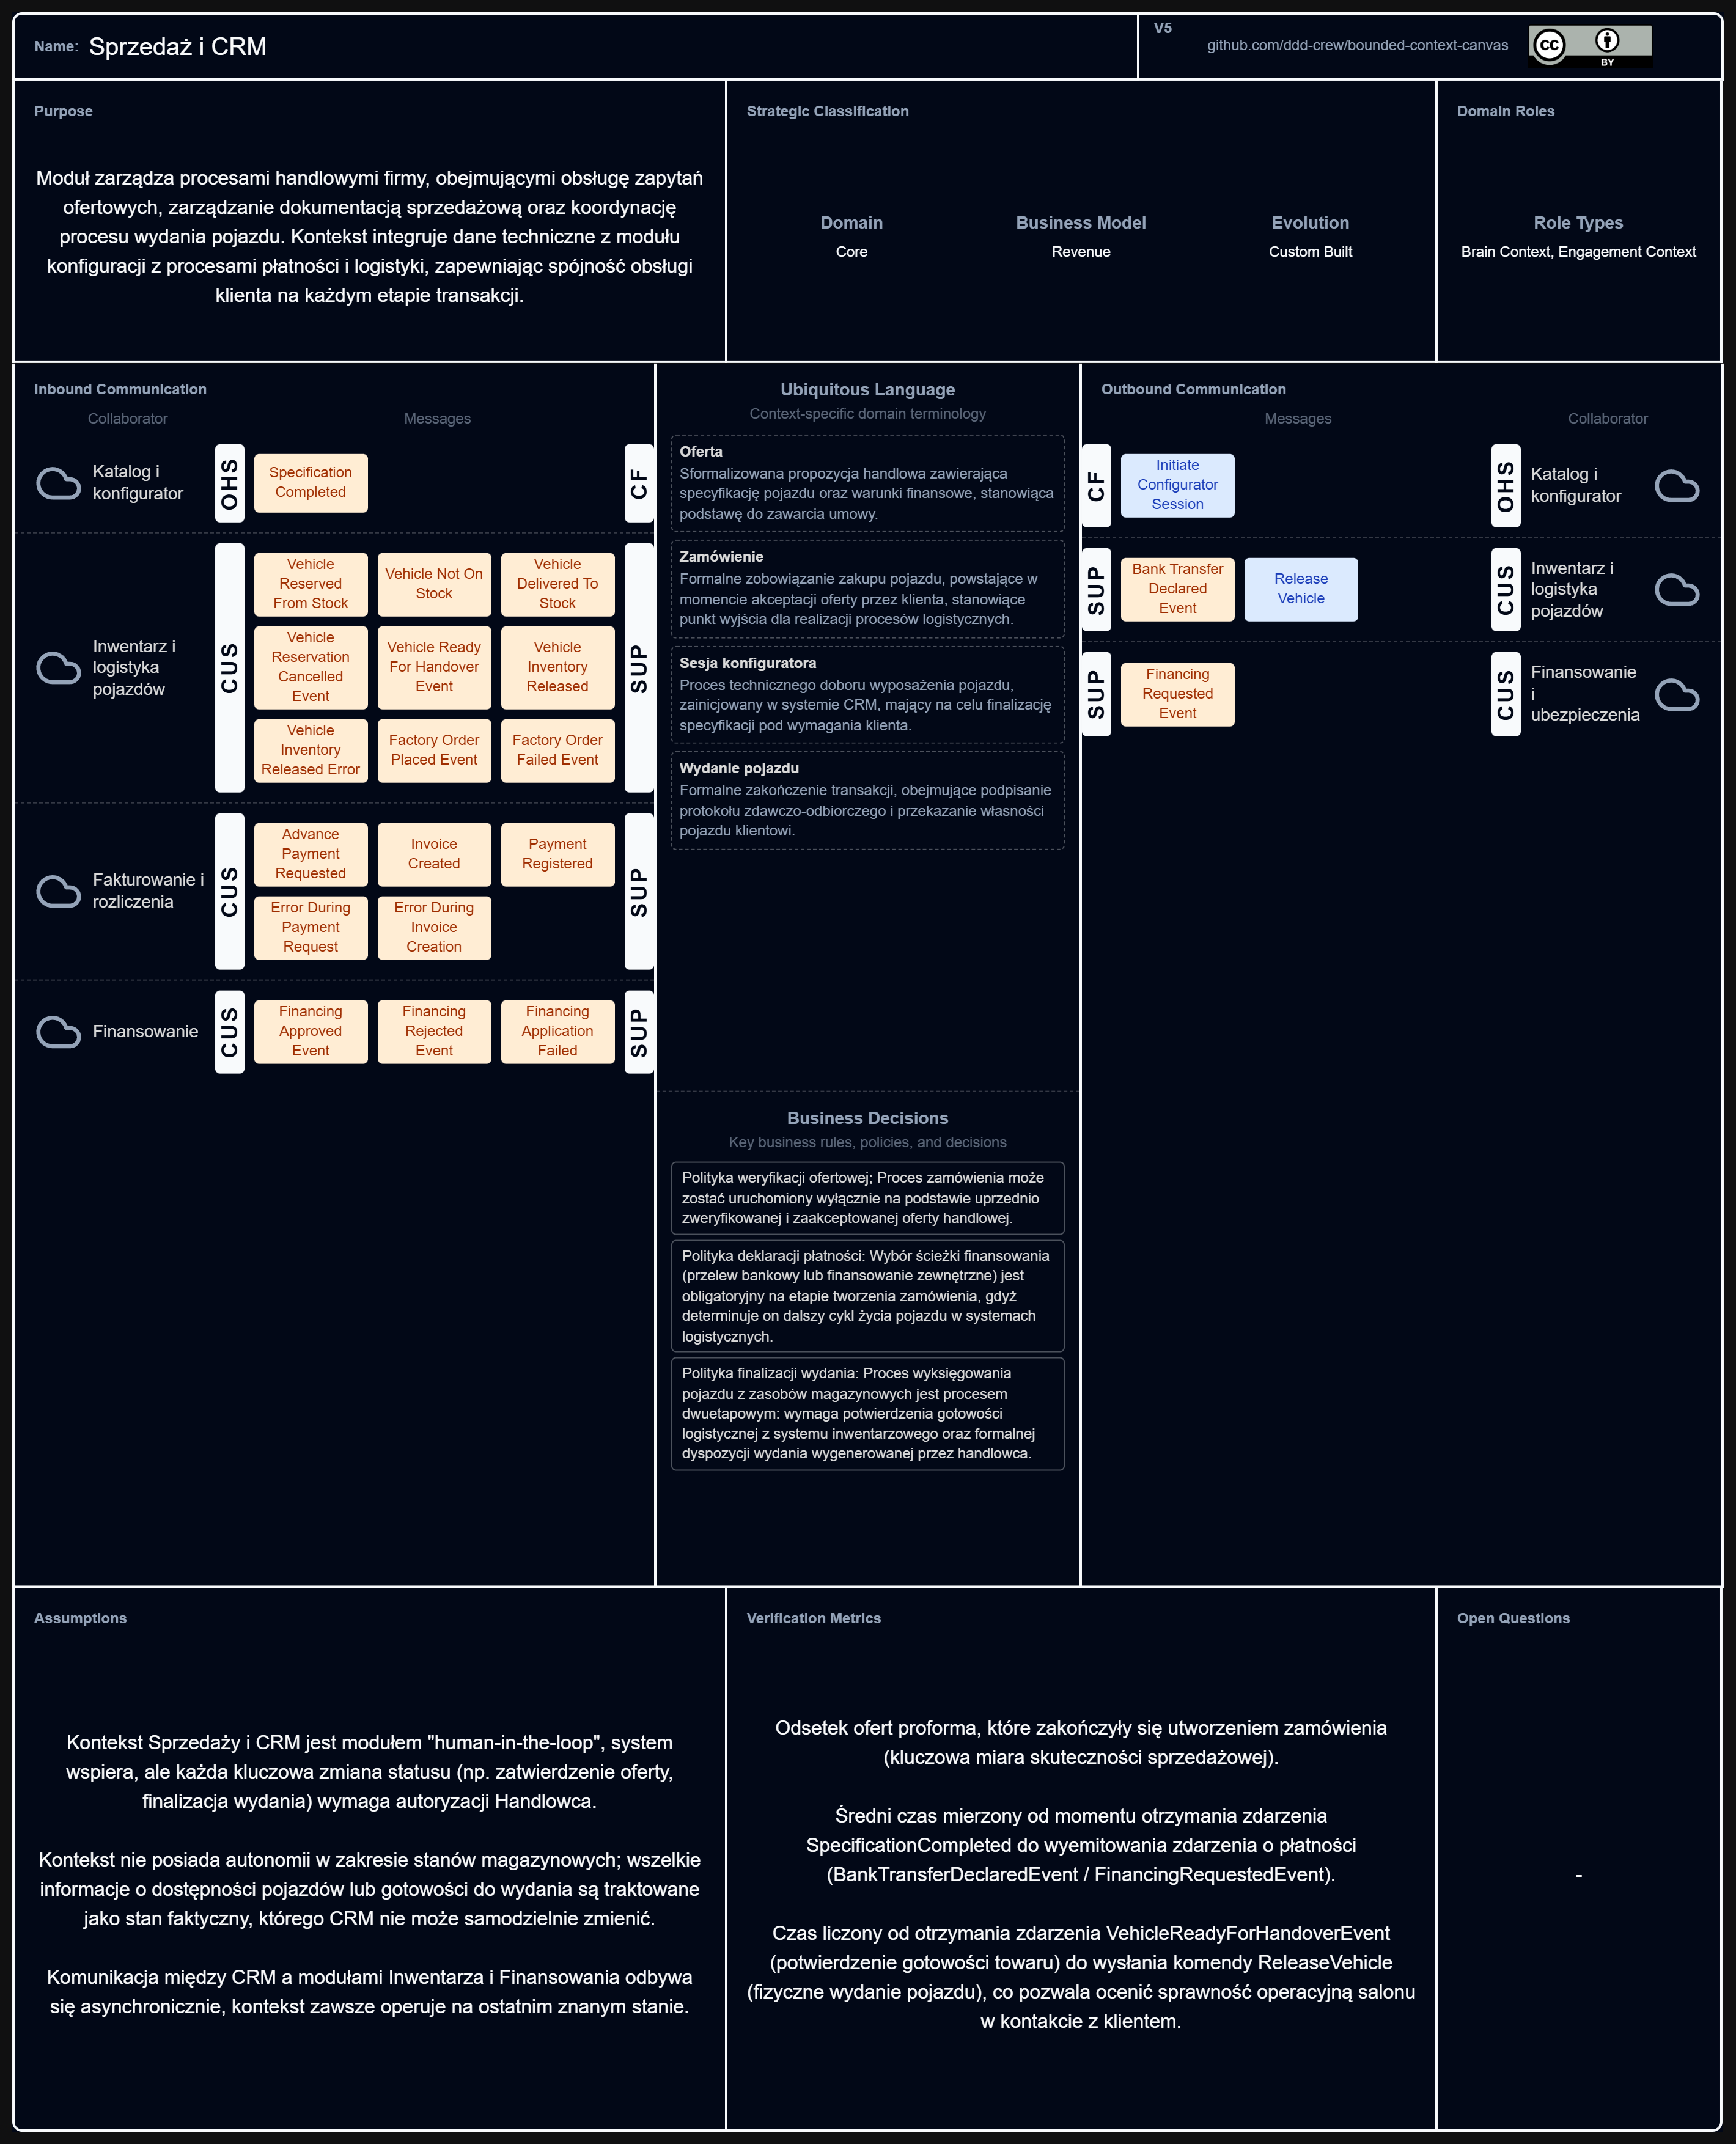
\includegraphics[width=\textwidth]{media/bounded-context-canvas/final/SIC_K1_TOTAL_FINAL.png}
    \caption{Kanwa Kontekstu Sprzedaży i CRM}
    \label{fig:hex_billing}
\end{figure}

\subsubsection{Przypadki użycia Kontekstu Sprzedaży}

% =====================================================
\textbf{UC-CRM-01: Uruchomienie sesji konfiguratora dla klienta}

\begin{longtable}{|p{4cm}|p{11cm}|}
\hline
\textbf{Element} & \textbf{Opis} \\
\hline

Identyfikator & UC-CRM-01 \\
\hline

Nazwa & Uruchomienie sesji konfiguratora dla klienta \\
\hline

Opis & 
Zainicjowanie procesu nowej sprzedaży poprzez wygenerowanie i otwarcie dedykowanej sesji w konfiguratorze pojazdów, przypisanej do konkretnego klienta i handlowca. \\
\hline

Aktor główny & Handlowiec \\
\hline

Aktorzy pomocniczy & - \\
\hline

Warunki wstępne & 
Klient wykazuje zainteresowanie zakupem nowego pojazdu. \\
\hline

Warunki końcowe & 
Wygenerowana zostaje nowa sesja, a kontekst emituje zdarzenie \textit{InitiateConfiguratorSession}. \\
\hline

Scenariusz główny & 
\begin{enumerate}
    \item Handlowiec wybiera opcję konfiguracji nowego pojazdu dla tego klienta.
    \item Kontekst emituje zdarzenie inicjujące \textit{InitiateConfiguratorSession}.
    \item System otwiera w nowym widoku interfejs konfiguratora (z modułu Katalogu).
\end{enumerate} \\
\hline

Scenariusze alternatywne & 
\begin{itemize}
    \item [] Brak.
\end{itemize} \\
\hline
\end{longtable}

\begin{figure}[H]
    \centering
    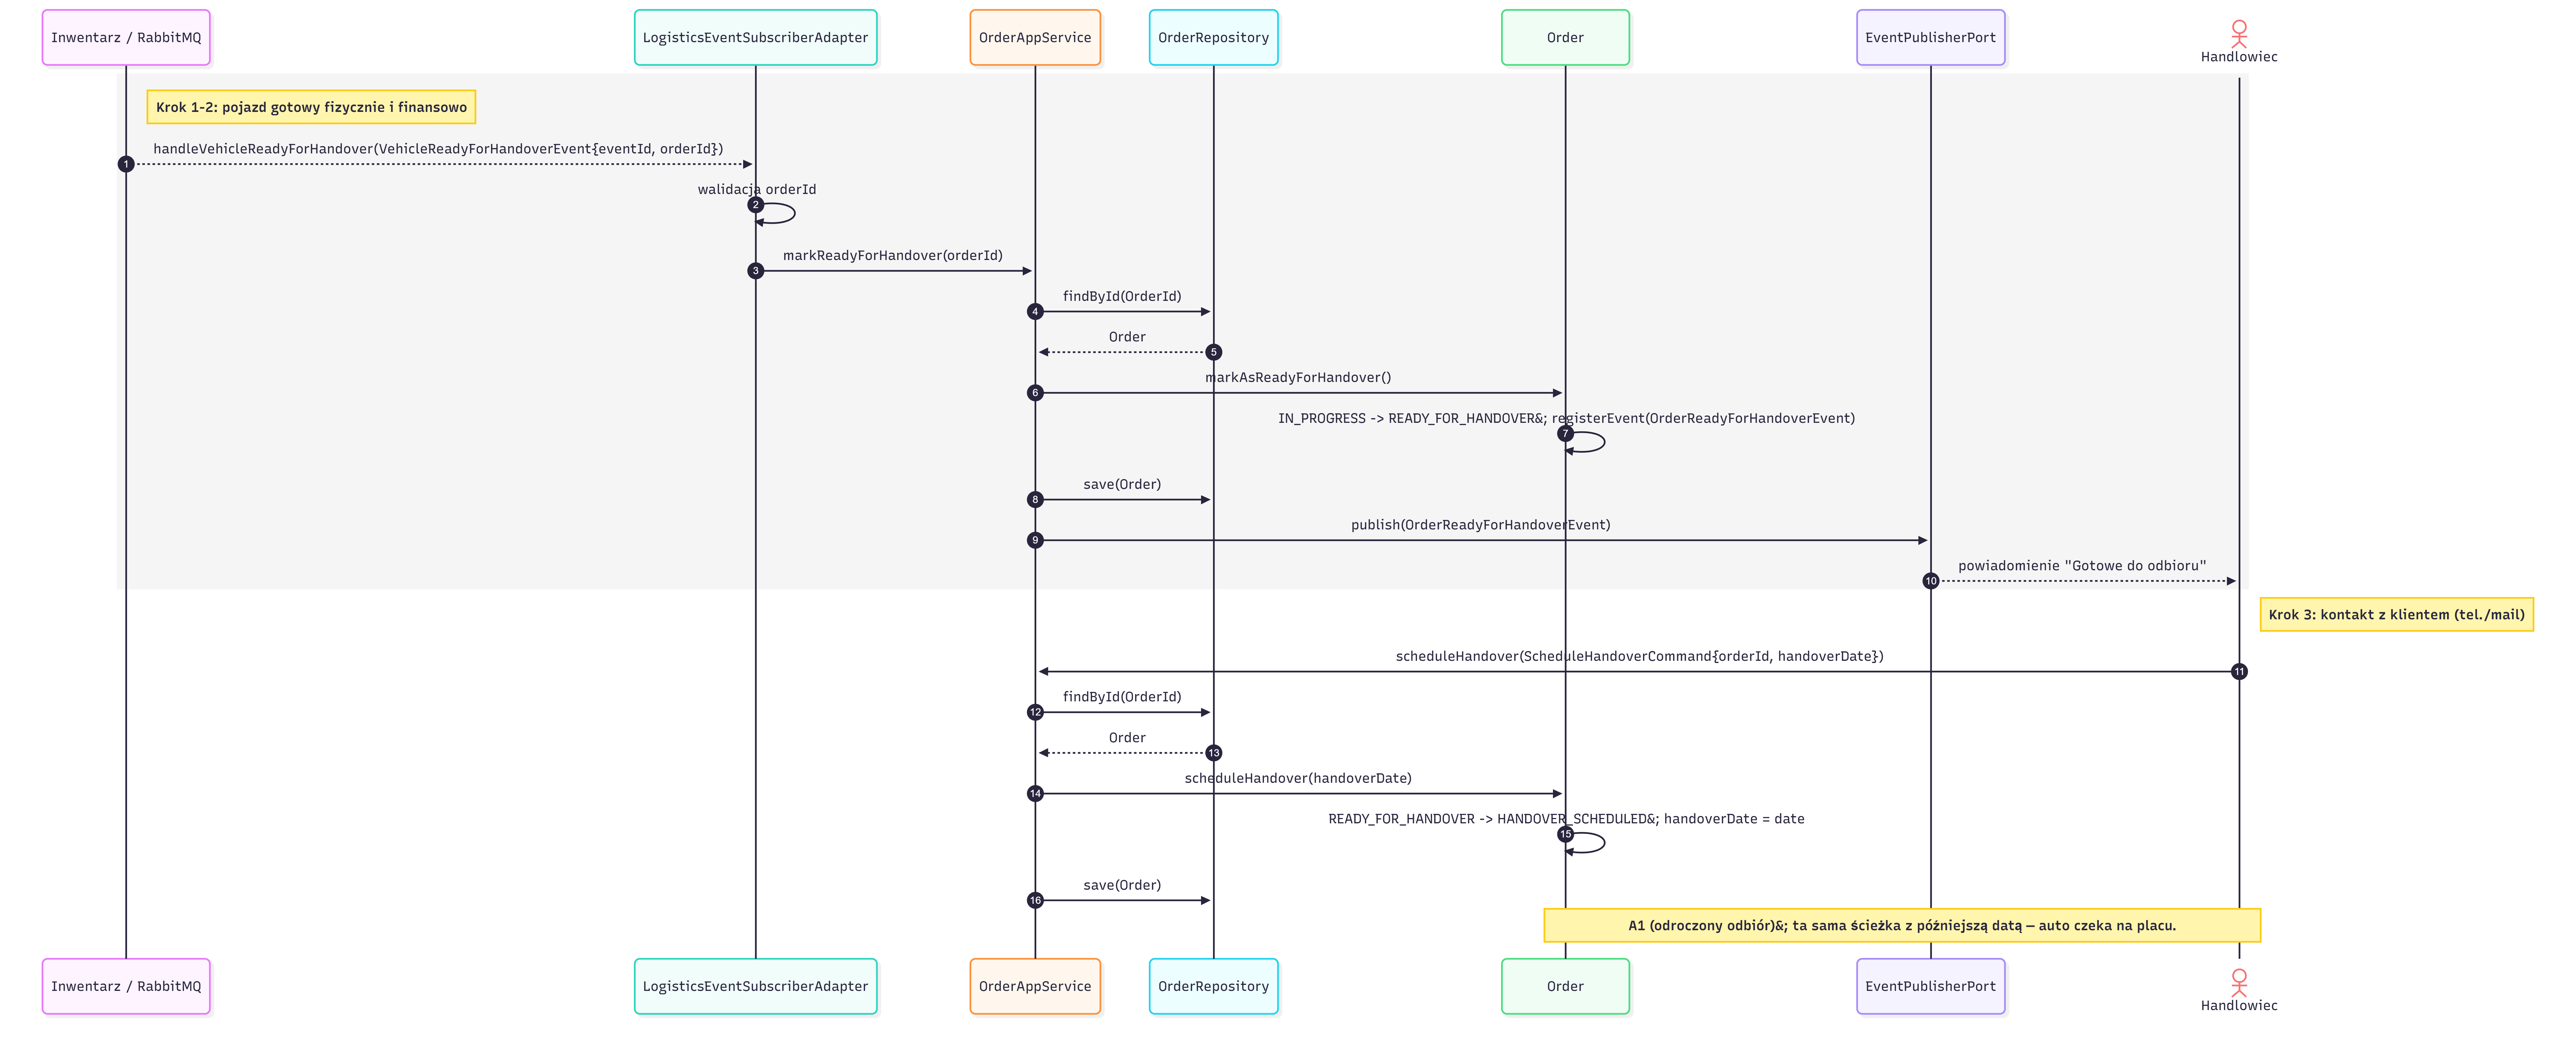
\includegraphics[width=1\textwidth]{media/diagramy_sekwencji/kontekst-sprzedazy/UC-CRM-01-Sekwencji.png}
    \caption{Diagram sekwencji dla przypadku użycia UC-CRM-01: Uruchomienie sesji konfiguratora dla klienta}
    \label{fig:seq_uc_crm_01}
\end{figure}

% =====================================================
\textbf{UC-CRM-02: Wygenerowanie oferty proforma}

\begin{longtable}{|p{4cm}|p{11cm}|}
\hline
\textbf{Element} & \textbf{Opis} \\
\hline

Identyfikator & UC-CRM-02 \\
\hline

Nazwa & Wygenerowanie oferty proforma \\
\hline

Opis & 
Proces utworzenia wstępnej oferty handlowej w systemie na podstawie danych (specyfikacji, ceny oraz danych kontaktowych klienta) otrzymanych od zdarzenia z konfiguratora. \\
\hline

Aktor główny & Handlowiec \\
\hline

Aktorzy pomocniczy & - \\
\hline

Warunki wstępne & 
Kontekst otrzymał zdarzenie \textit{SpecificationCompleted} zawierające pełną konfigurację, wyliczoną cenę oraz dane identyfikacyjne klienta. \\
\hline

Warunki końcowe & 
Nowa Oferta zostaje utworzona i zapisana w systemie ze statusem "W przygotowaniu". \\
\hline

Scenariusz główny & 
\begin{enumerate}
    \item System powiadamia handlowca o nowej specyfikacji oczekującej na ofertowanie.
    \item Handlowiec otwiera formularz nowej oferty.
    \item Handlowiec uzupełnia ofertę o dane klienta. Informacje o specyfikacji i cenie katalogowej uzupełniane są bezpośrednio z otrzymanego zdarzenia.
    \item Handlowiec generuje dokument oferty proforma zmieniając status na 'Utworzona' i prezentuje go klientowi.
\end{enumerate} \\
\hline

Scenariusze alternatywne & 
\begin{itemize}
    \item [] Brak.
\end{itemize} \\
\hline
\end{longtable}

\begin{figure}[H]
    \centering
    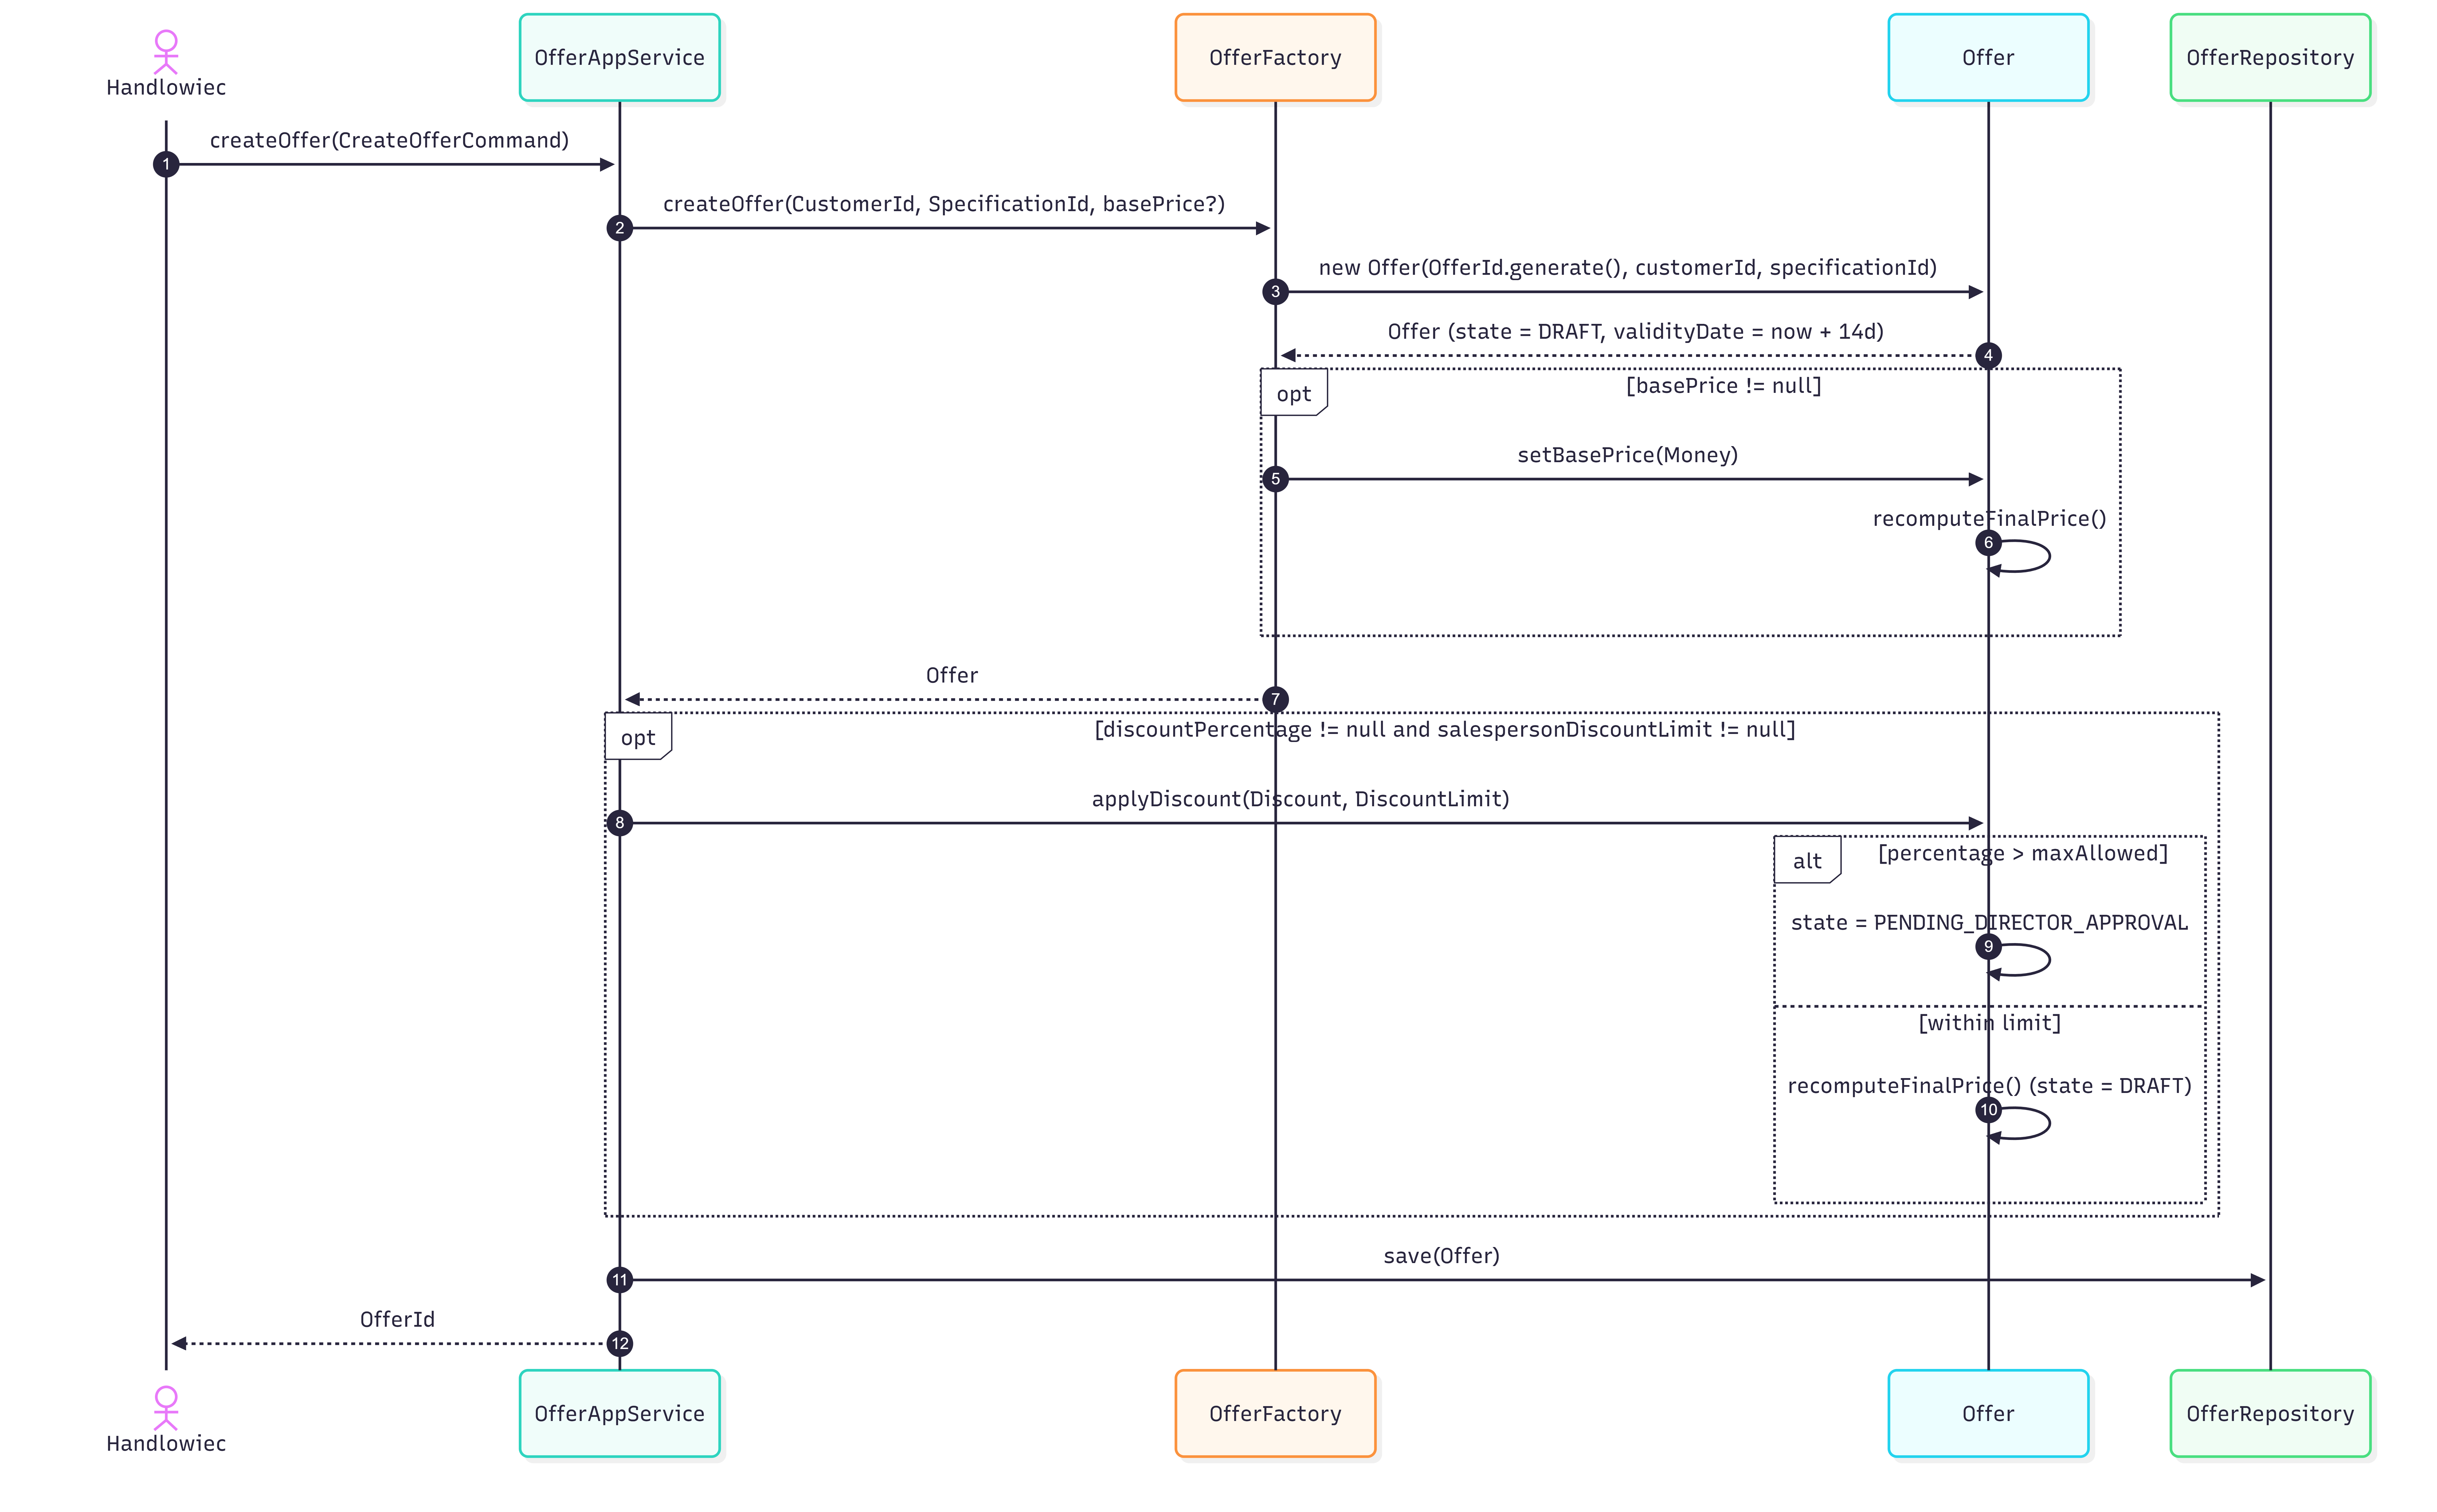
\includegraphics[width=1\textwidth]{media/diagramy_sekwencji/kontekst-sprzedazy/UC-CRM-02-Sekwencji.png}
    \caption{Diagram sekwencji dla przypadku użycia UC-CRM-02: Wygenerowanie oferty proforma}
    \label{fig:seq_uc_crm_02}
\end{figure}

% =====================================================
\textbf{UC-CRM-03: Zatwierdzenie oferty i utworzenie zamówienia}

\begin{longtable}{|p{4cm}|p{11cm}|}
\hline
\textbf{Element} & \textbf{Opis} \\
\hline

Identyfikator & UC-CRM-03 \\
\hline

Nazwa & Zatwierdzenie oferty, utworzenie zamówienia i wybór formy płatności \\
\hline

Opis & 
Proces akceptacji wygenerowanej oferty przez klienta oraz utworzenia na jej podstawie nowego zamówienia (osobnego agregatu), co uruchamia właściwe procesy logistyczne i sprzedażowe. \\
\hline

Aktor główny & Handlowiec \\
\hline

Aktorzy pomocniczy & Klient \\
\hline

Warunki wstępne & 
Wygenerowana i ważna oferta proforma (agregat Oferta) istnieje w systemie CRM. \\
\hline

Warunki końcowe & 
Oferta otrzymuje status "Zaakceptowana". W systemie powstaje nowe Zamówienie ze statusem "W realizacji", a system emituje odpowiednie zdarzenie inicjujące weryfikację stanu magazynowego placu lub proces bankowy. \\
\hline

Scenariusz główny & 
\begin{enumerate}
    \item Klient akceptuje warunki przedstawione na ofercie proforma.
    \item Handlowiec zmienia status oferty na "Zaakceptowana" w systemie CRM.
    \item Handlowiec tworzy nowe zamówienie na podstawie zaakceptowanej oferty.
    \item Handlowiec wprowadza na zamówieniu zadeklarowaną przez klienta formę płatności (Przelew lub Finansowanie).
    \item System CRM emituje zdarzenie \textit{BankTransferDeclaredEvent} (dla przelewu) LUB \textit{FinancingRequestedEvent} (dla finansowania).
\end{enumerate} \\
\hline

Scenariusze alternatywne & 
\begin{itemize}
    \item [A1] Klient odrzuca ofertę: W kroku 1 klient rezygnuje. Handlowiec zmienia status oferty na "Odrzucona". Nowe zamówienie nie powstaje, a żadne zdarzenie biznesowe nie jest emitowane do innych modułów.
\end{itemize} \\
\hline
\end{longtable}

\begin{figure}[H]
    \centering
    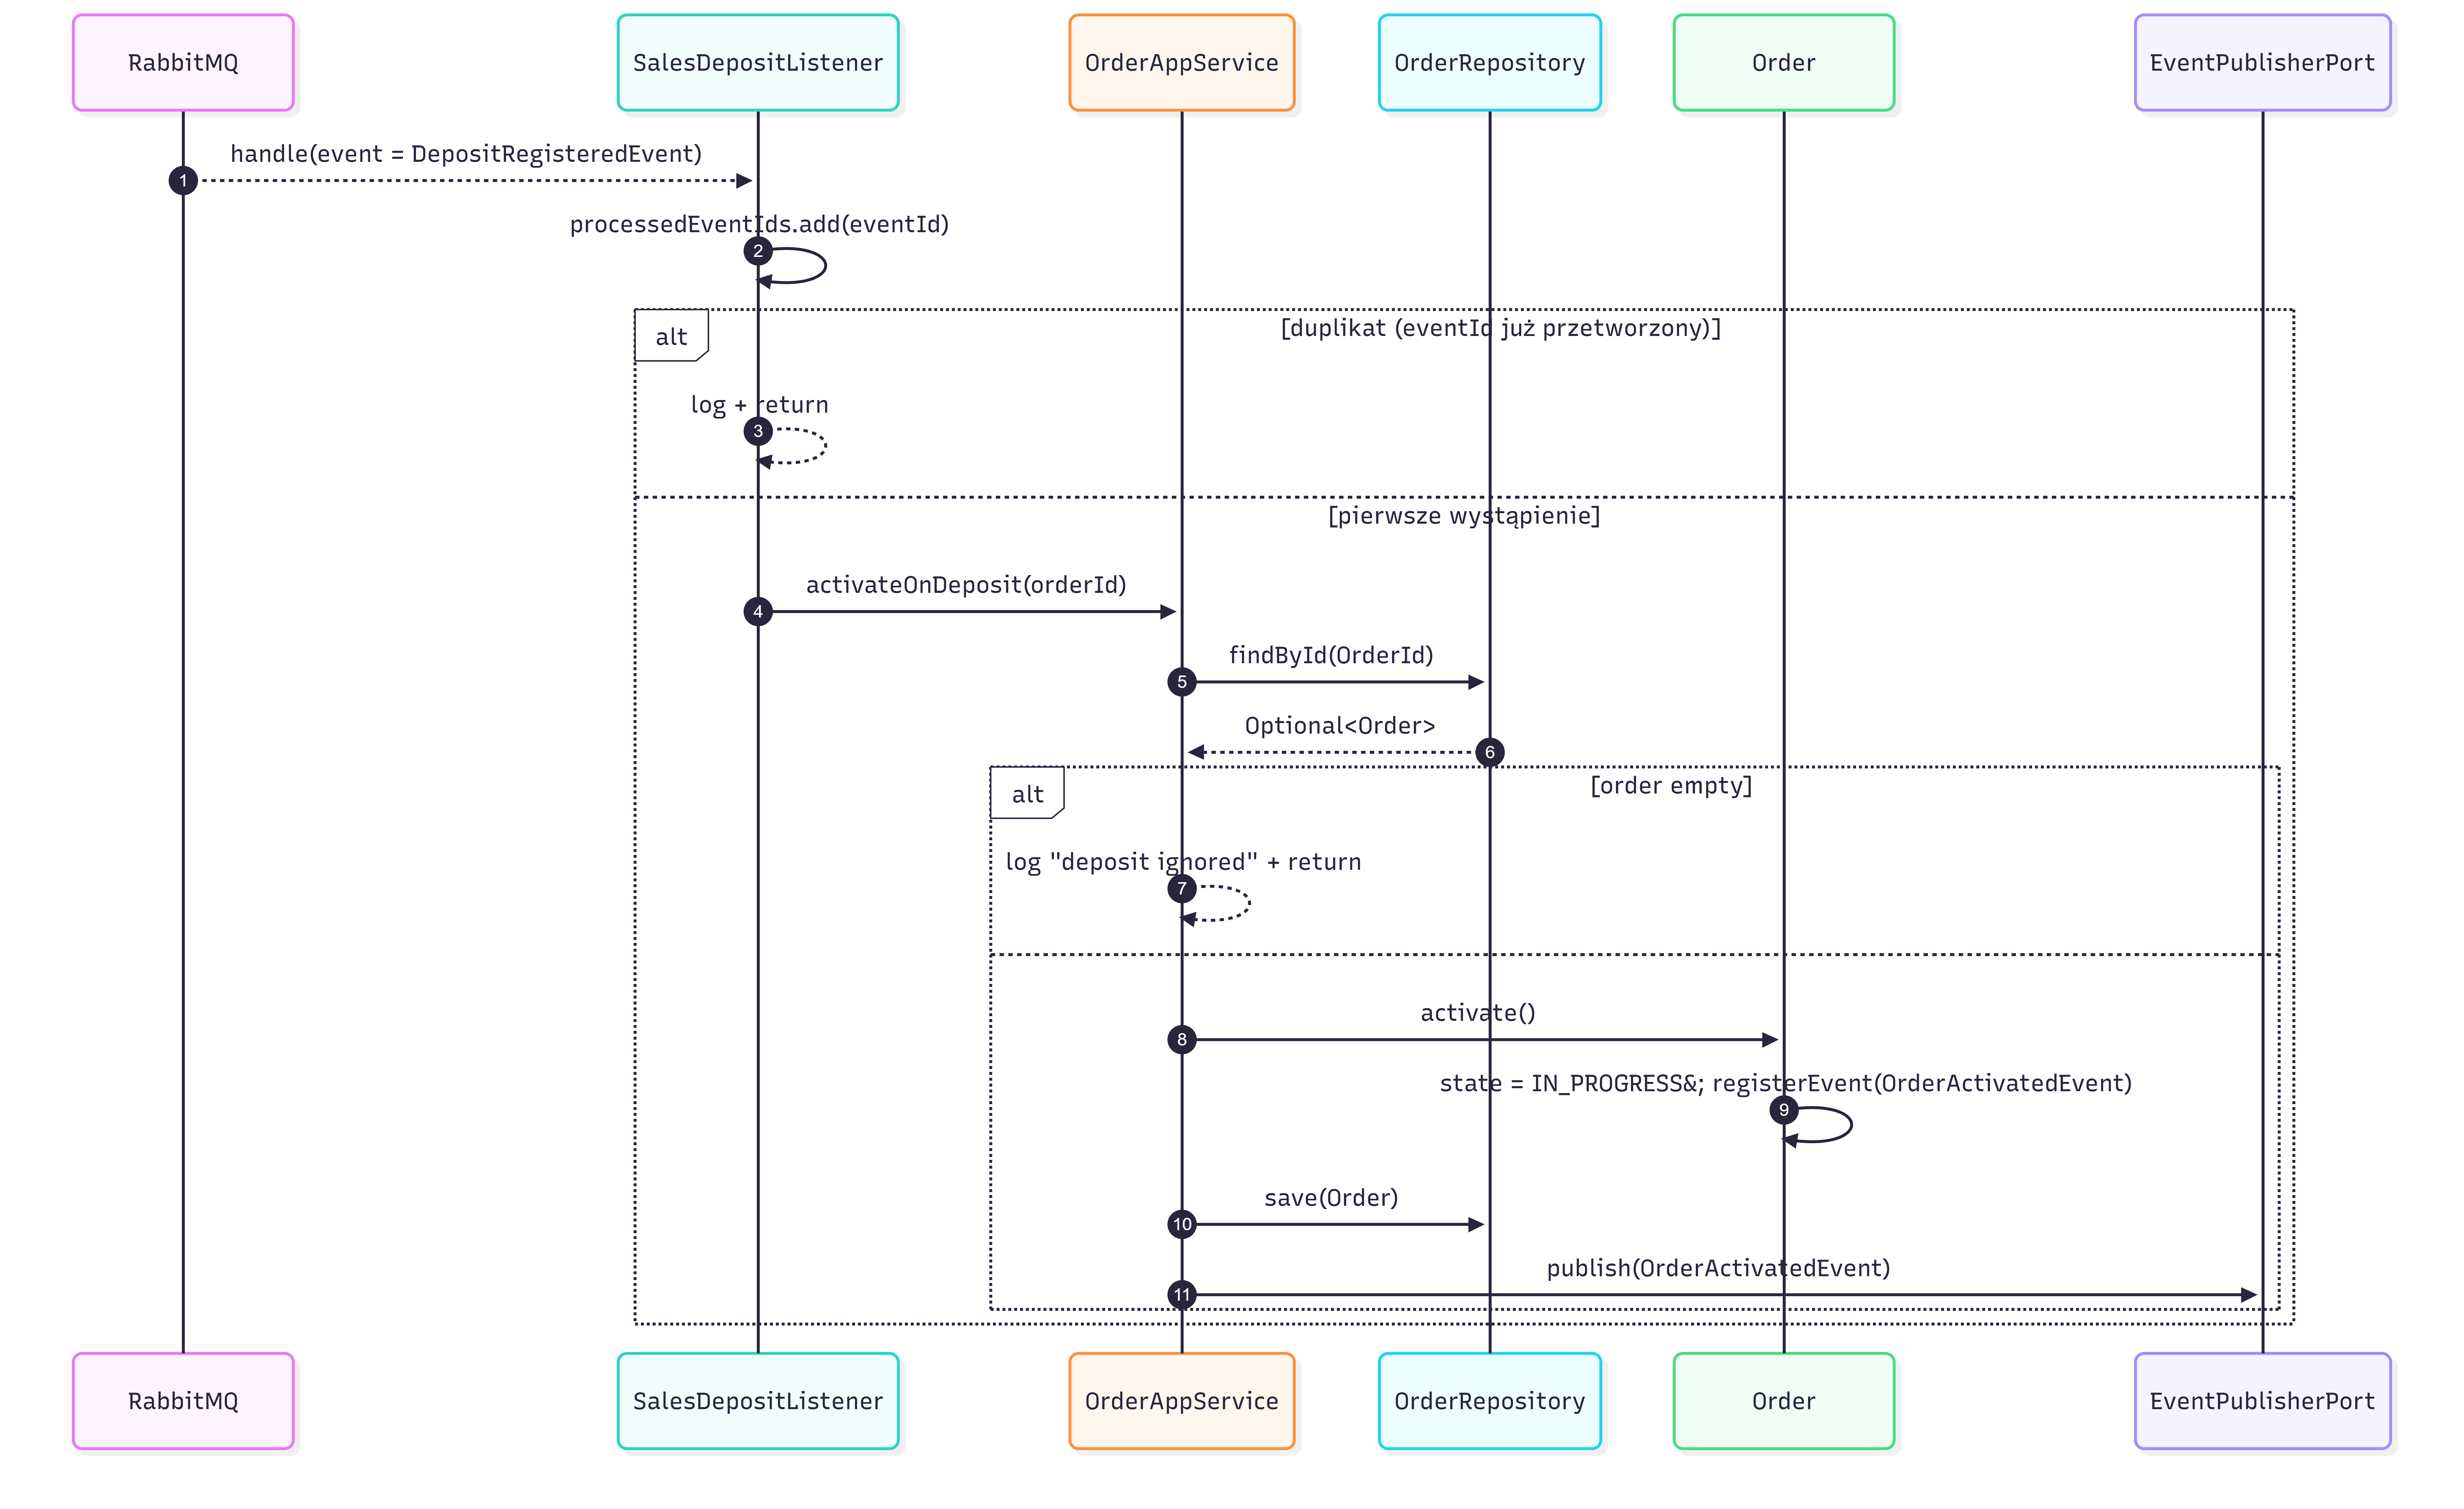
\includegraphics[width=1\textwidth]{media/diagramy_sekwencji/kontekst-sprzedazy/UC-CRM-03(cz2)-Sekwencji.png}
    \caption{Diagram sekwencji dla przypadku użycia UC-CRM-03 (cz.1): Konwersja oferty w zamówienie}
    \label{fig:seq_uc_crm_03cz1}
\end{figure}

\begin{figure}[H]
    \centering
    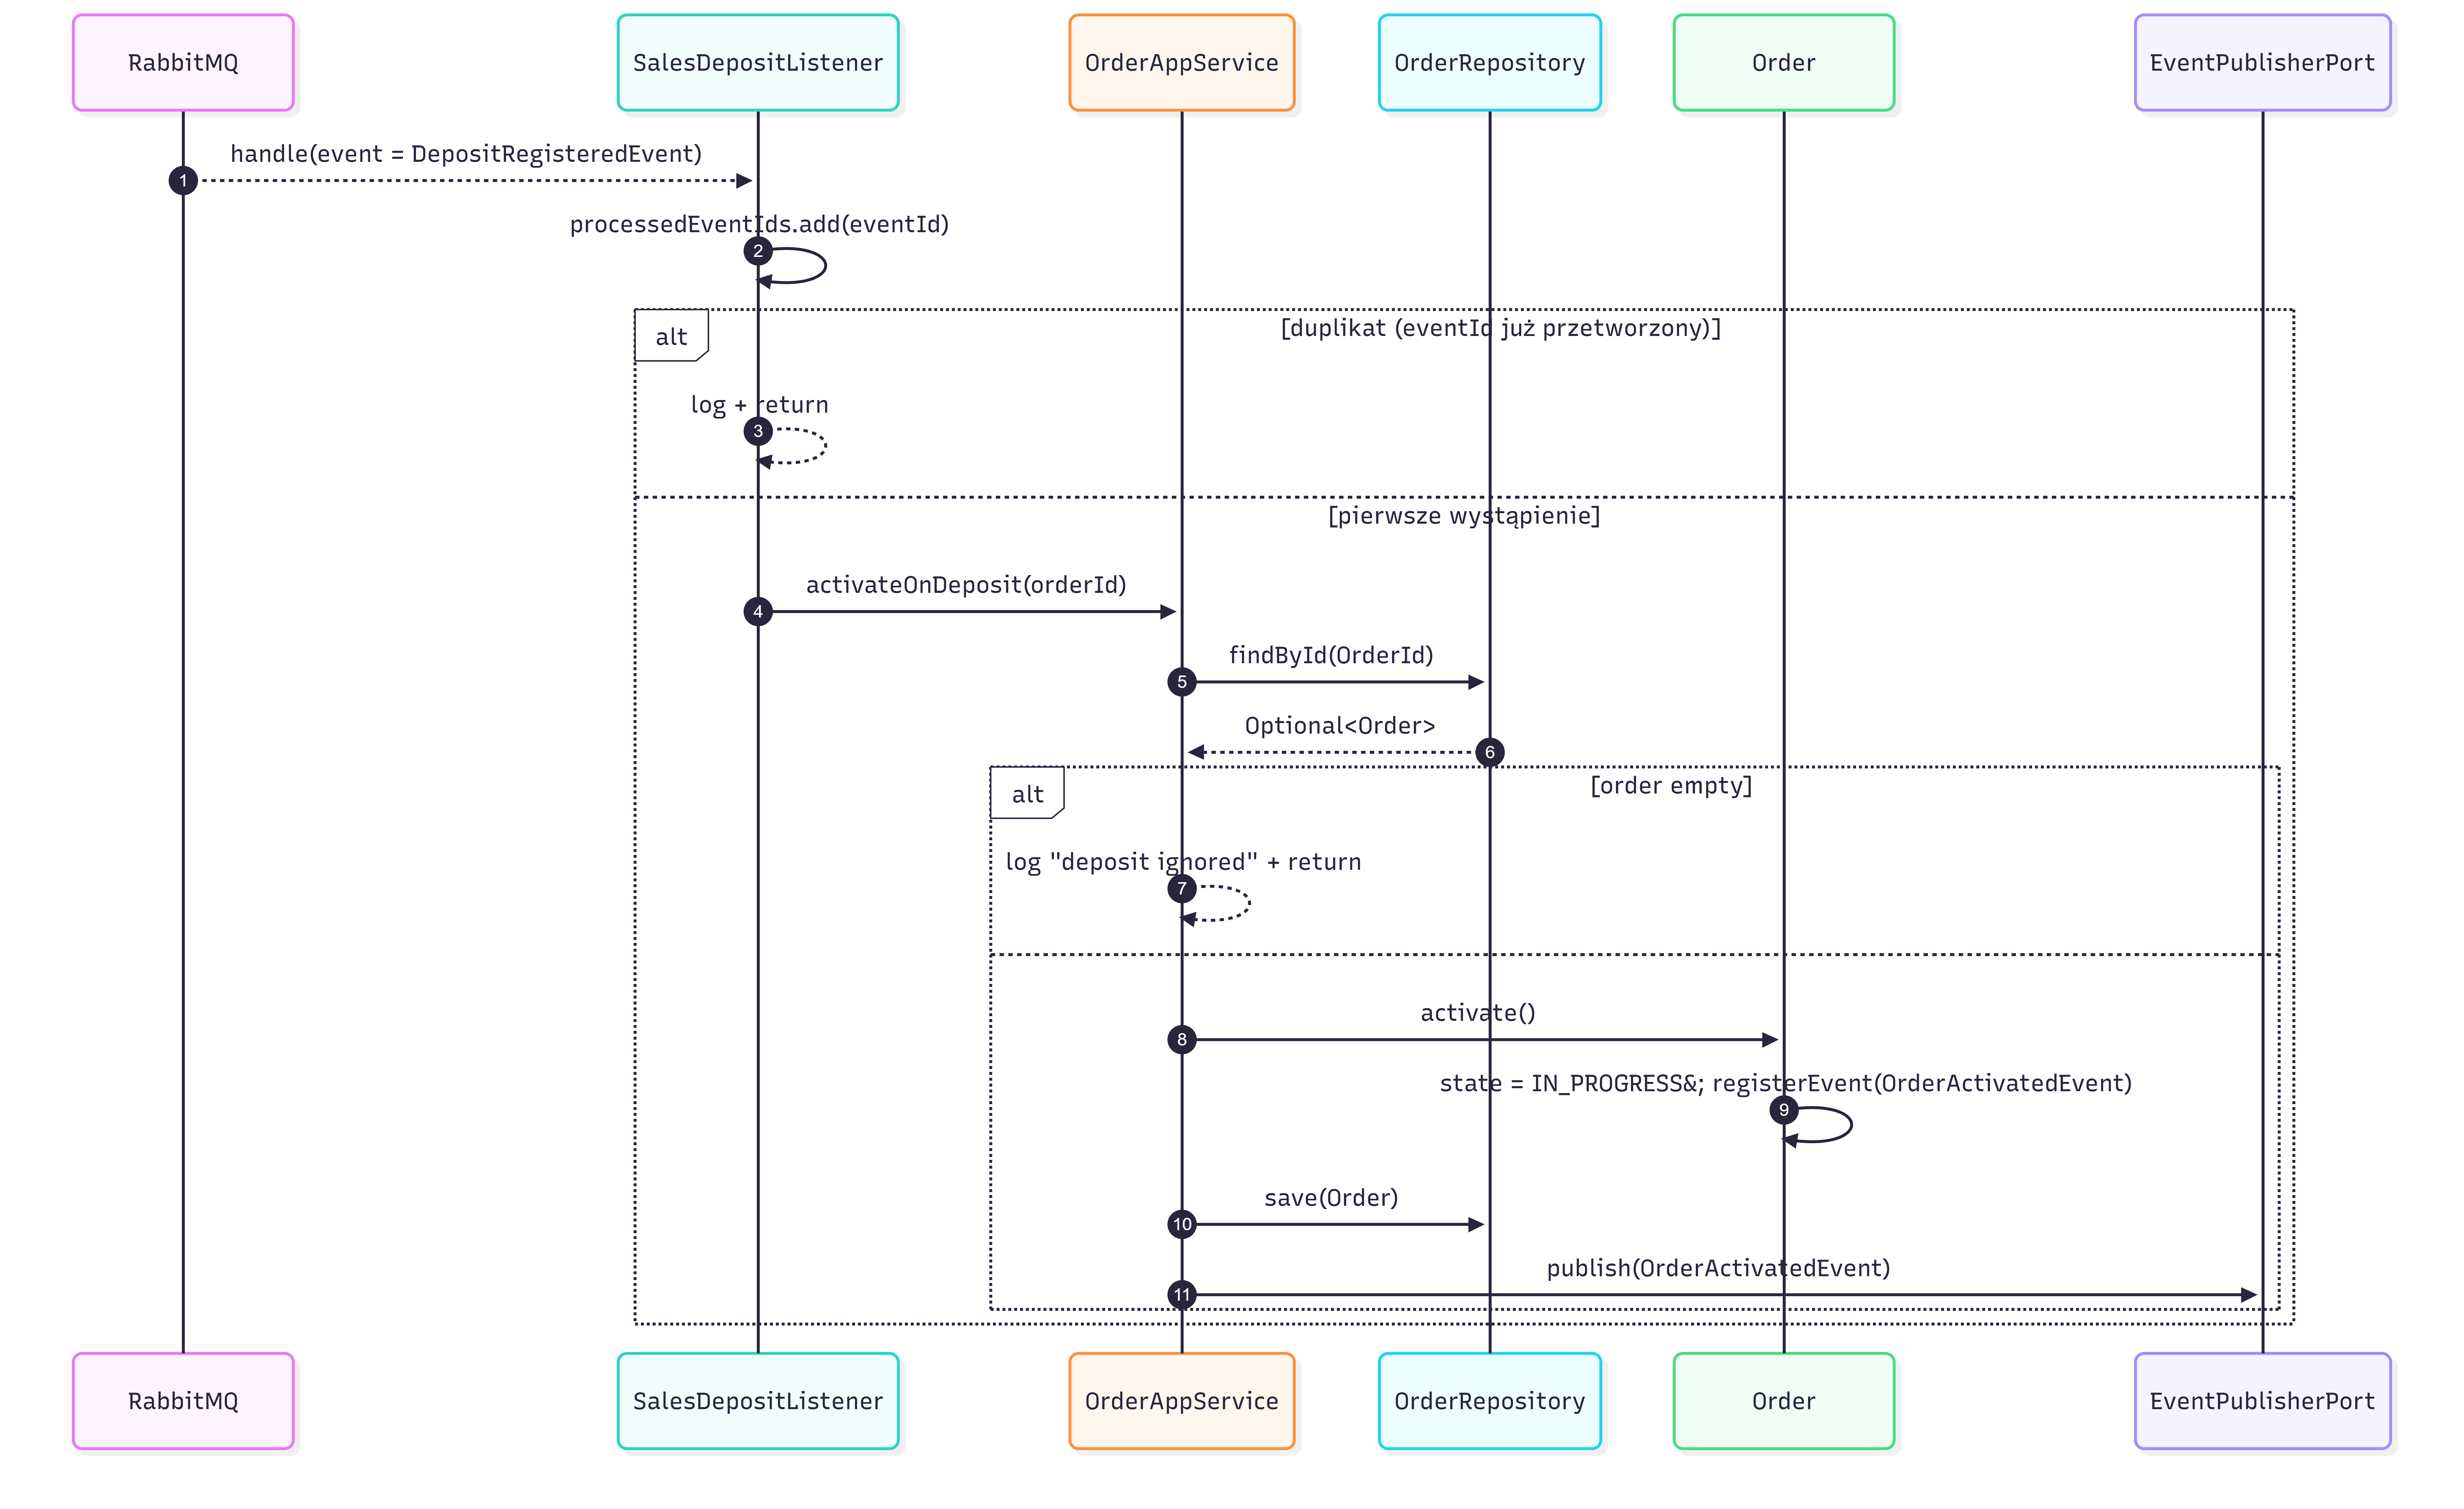
\includegraphics[width=1\textwidth]{media/diagramy_sekwencji/kontekst-sprzedazy/UC-CRM-03(cz2)-Sekwencji.png}
    \caption{Diagram sekwencji dla przypadku użycia  UC-CRM-03 (cz.2): Aktywacja po zadatku}
    \label{fig:seq_uc_crm_03cz2}
\end{figure}

% =====================================================
\textbf{UC-CRM-04: Obsługa zaproszenia klienta po odbiór}

\begin{longtable}{|p{4cm}|p{11cm}|}
\hline
\textbf{Element} & \textbf{Opis} \\
\hline

Identyfikator & UC-CRM-04 \\
\hline

Nazwa & Obsługa zaproszenia klienta po odbiór \\
\hline

Opis & 
Reakcja systemu na sygnał o pełnej gotowości fizycznej i finansowej pojazdu, uruchamiająca proces kontaktu z klientem w celu zaplanowania wydania auta. \\
\hline

Aktor główny & Handlowiec \\
\hline

Aktorzy pomocniczy & - \\
\hline

Warunki wstępne & 
Kontekst otrzymał zdarzenie \textit{VehicleReadyForHandoverEvent}. \\
\hline

Warunki końcowe & 
Ustalenie daty odbioru pojazdu i aktualizacja statusu zamówienia w CRM na "Umówiony na odbiór". \\
\hline

Scenariusz główny & 
\begin{enumerate}
    \item Kontekst sprzedaży i CRM odbiera zdarzenie \textit{VehicleReadyForHandoverEvent}.
    \item System zmienia status zamówienia na "Gotowe do odbioru" i generuje powiadomienie dla Handlowca.
    \item Handlowiec kontaktuje się z klientem (telefonicznie lub mailowo).
    \item Handlowiec wprowadza do systemu uzgodnioną z klientem datę i godzinę odbioru pojazdu.
    \item System aktualizuje status zamówienia na "Umówiony na odbiór".
\end{enumerate} \\
\hline

Scenariusze alternatywne & 
\begin{itemize}
    \item [A1] Odroczony odbiór: W kroku 3 klient informuje, że nie może odebrać auta w najbliższych dniach. Handlowiec ustawia odroczony termin w systemie, auto czeka na placu.
\end{itemize} \\
\hline
\end{longtable}

\begin{figure}[H]
    \centering
    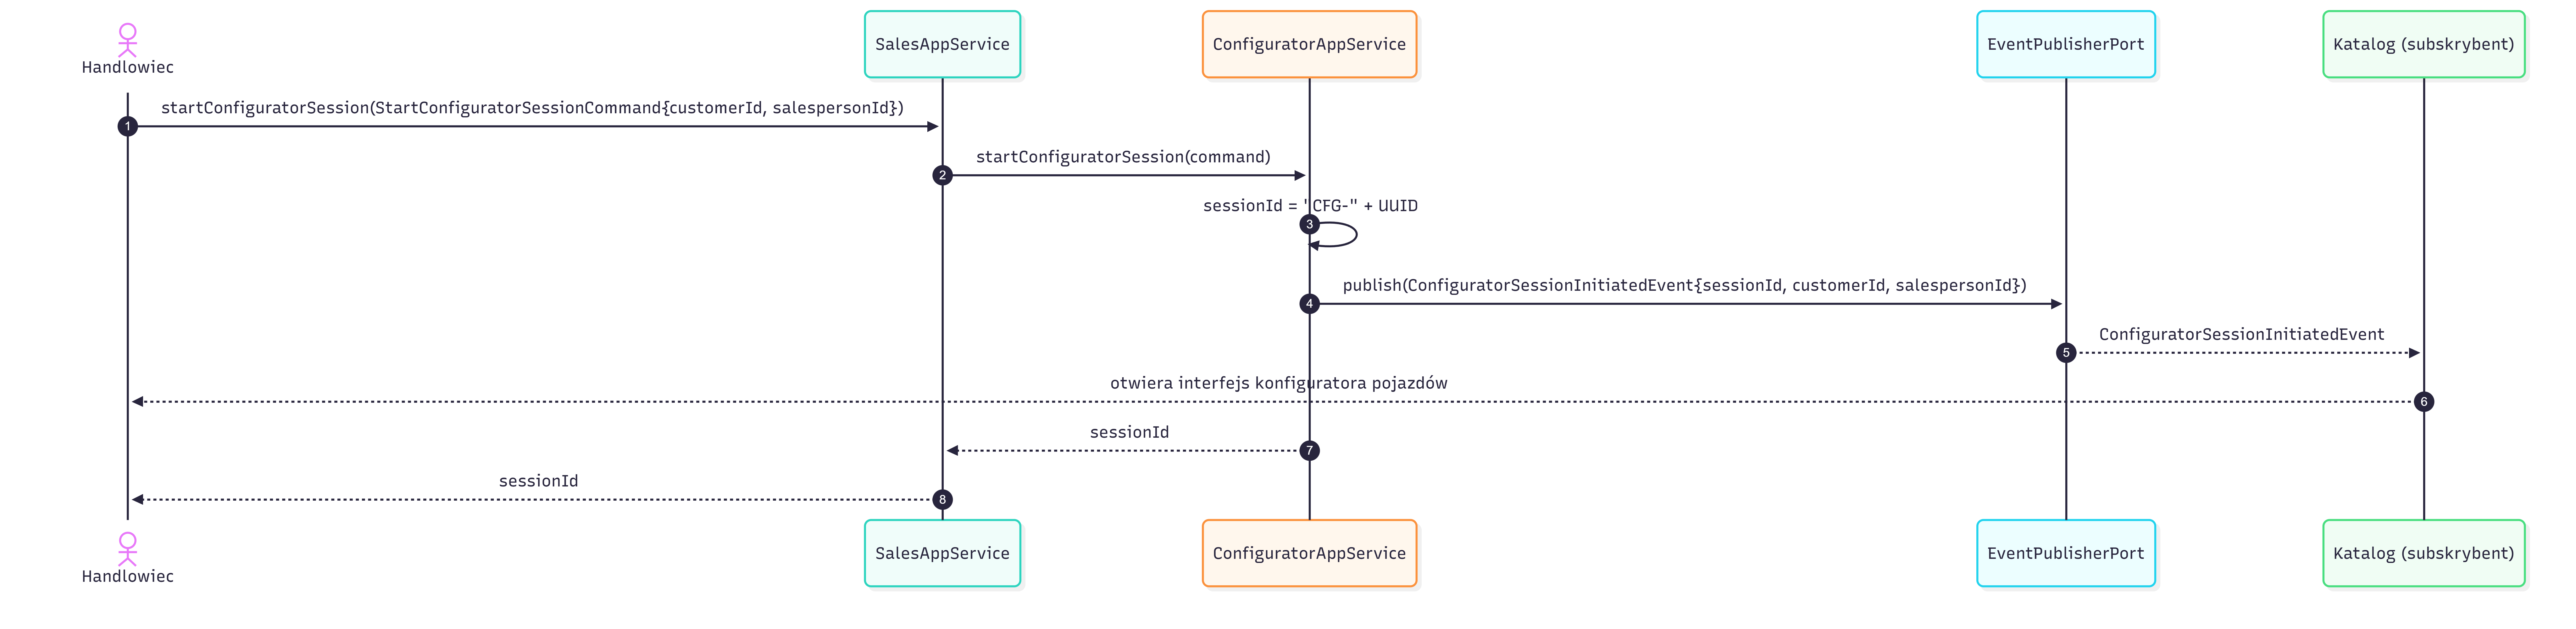
\includegraphics[width=1\textwidth]{media/diagramy_sekwencji/kontekst-sprzedazy/UC-CRM-04-Sekwencji.png}
    \caption{Diagram sekwencji dla przypadku użycia UC-CRM-04: Obsługa zaproszenia klienta po odbiór}
    \label{fig:seq_uc_crm_04}
\end{figure}

% =====================================================
\textbf{UC-CRM-05: Rejestracja fizycznego wydania pojazdu}

\begin{longtable}{|p{4cm}|p{11cm}|}
\hline
\textbf{Element} & \textbf{Opis} \\
\hline

Identyfikator & UC-CRM-05 \\
\hline

Nazwa & Rejestracja fizycznego wydania pojazdu \\
\hline

Opis & 
Finalny krok w procesie sprzedaży, zamykający transakcję i uruchamiający systemowe zwolnienie pojazdu. \\
\hline

Aktor główny & Handlowiec \\
\hline

Aktorzy pomocniczy & - \\
\hline

Warunki wstępne & 
Zamówienie posiada status "Umówiony na odbiór", klient stawił się w salonie. \\
\hline

Warunki końcowe & 
Zamówienie otrzymuje status "Zrealizowane", a CRM wysyła komendę \textit{ReleaseVehicle} do Inwentarza. \\
\hline

Scenariusz główny & 
\begin{enumerate}
    \item Handlowiec przeprowadza z klientem formalności papierowe i podpisuje protokół wydania.
    \item Handlowiec klika w systemie CRM przycisk potwierdzający wydanie pojazdu.
    \item Kontekst CRM wysyła komendę \textit{ReleaseVehicle} do modułu Inwentarza.
    \item System oznacza zamówienie jako 'Zrealizowane'.
\end{enumerate} \\
\hline

Scenariusze alternatywne & 
\begin{itemize}
    \item [A1] Odmowa Inwentarza: Po kroku 3 kontekst CRM odbiera z Inwentarza zdarzenie błędu \textit{VehicleInventoryReleasedError}. System wyświetla handlowcowi powiadomienie o blokadzie magazynowej i cofa zamówienie do statusu "Gotowe do odbioru".
\end{itemize} \\
\hline
\end{longtable}

\begin{figure}[H]
    \centering
    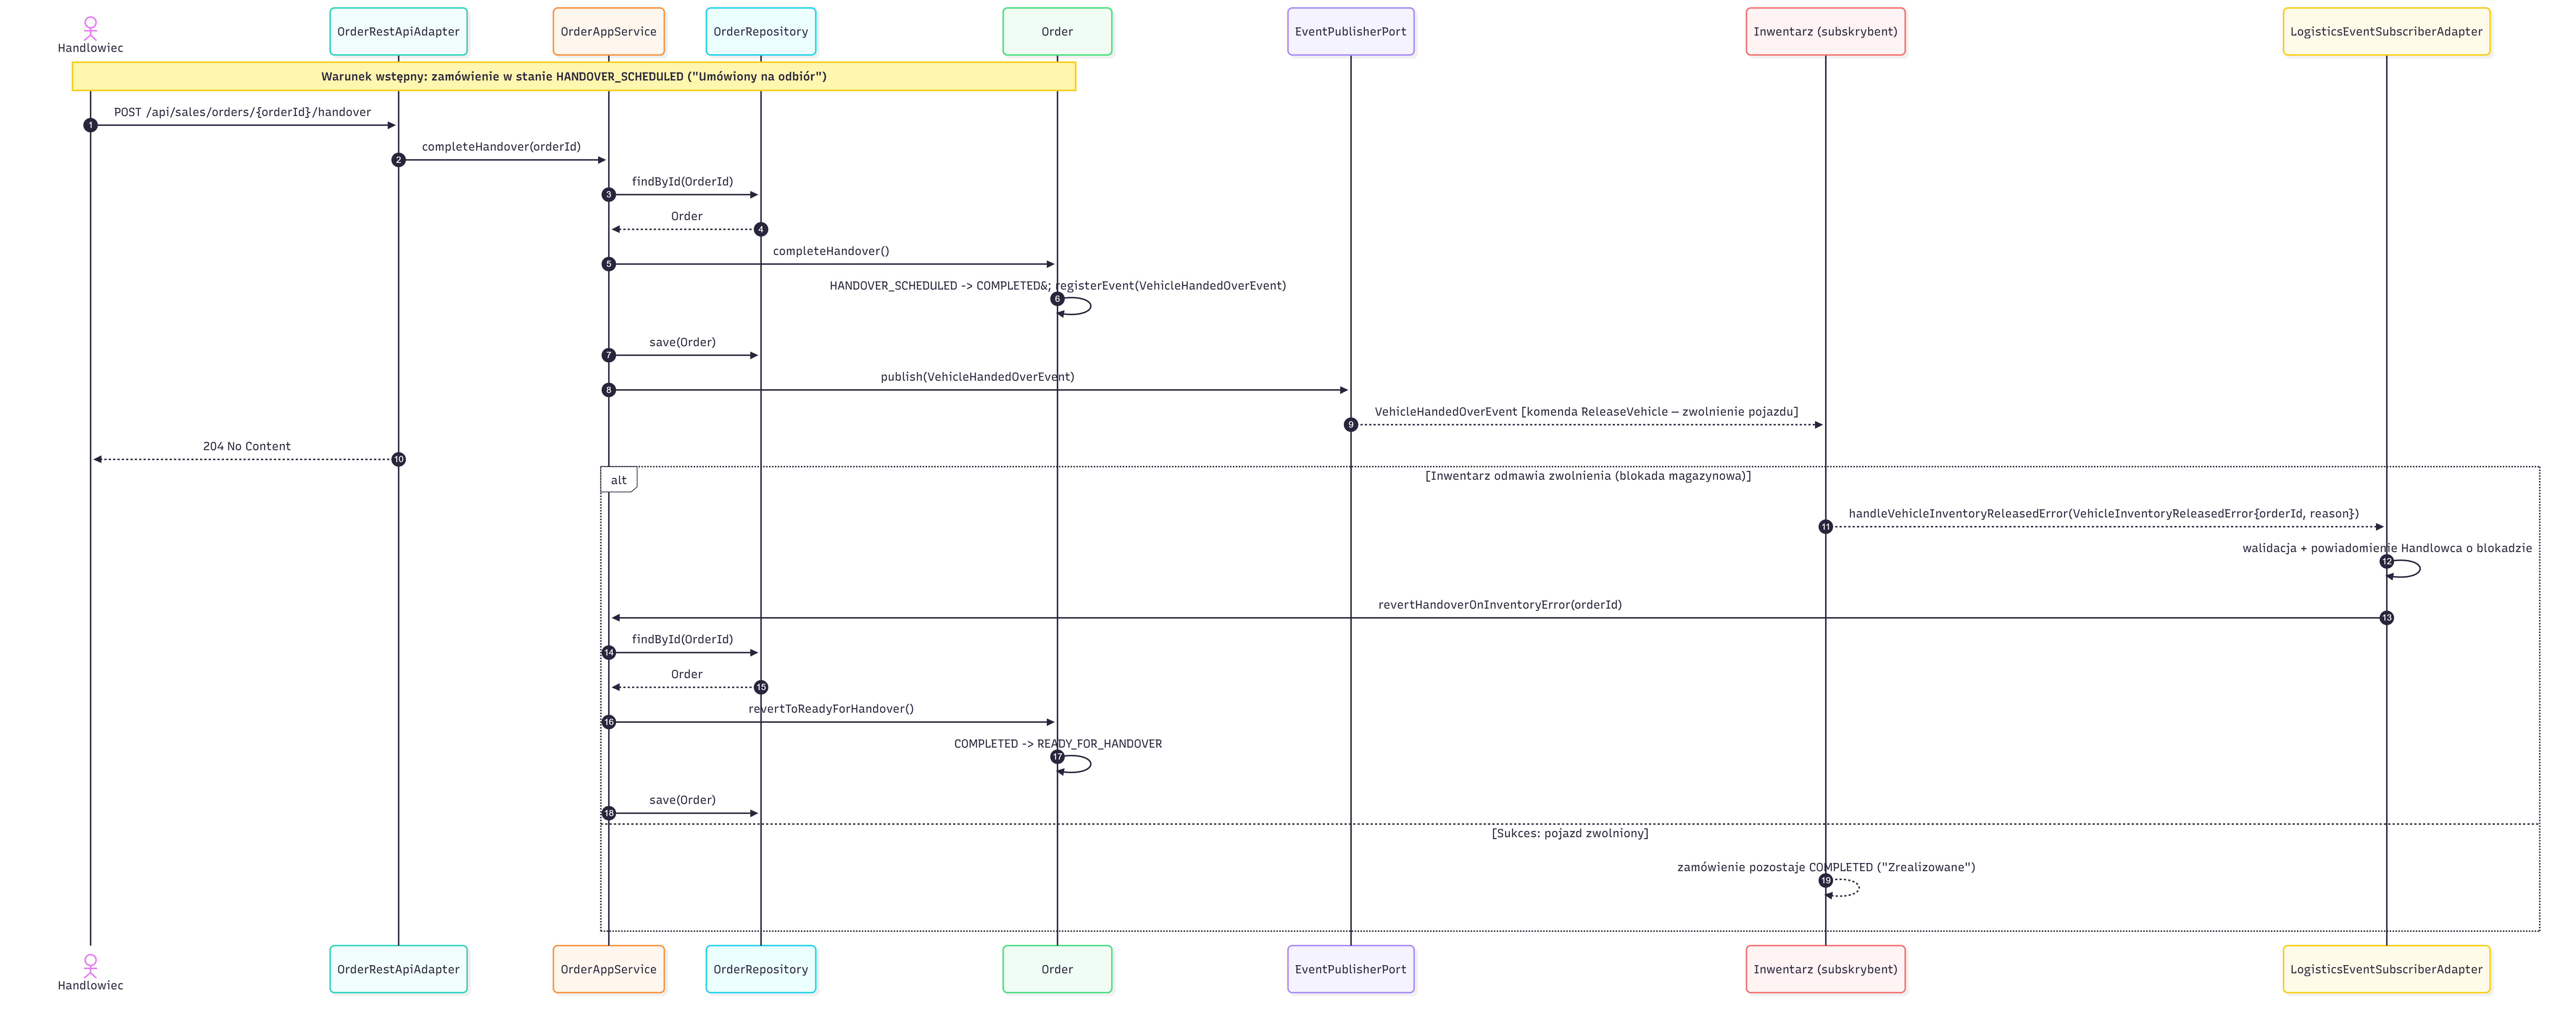
\includegraphics[width=1\textwidth]{media/diagramy_sekwencji/kontekst-sprzedazy/UC-CRM-05-Sekwencji.png}
    \caption{Diagram sekwencji dla przypadku użycia UC-CRM-05: Rejestracja fizycznego wydania pojazdu}
    \label{fig:seq_uc_crm_05}
\end{figure}

\subsubsection{Architektura Kontekstu Sprzedaży}

Kontekst Sprzedaży i CRM stanowi centralny węzeł operacyjny systemu, orkiestrujący pełen proces obsługi klienta – od inicjacji konfiguracji, aż po finalne wydanie pojazdu. Ze względu na wysoką złożoność biznesową i konieczność integracji z licznymi modułami zewnętrznymi, architekturę oparto na usłudze aplikacyjnej obsługi sprzedaży (\texttt{SalesService}), uzupełnionej o \texttt{ConfiguratorAppService} (sesje konfiguratora) i \texttt{SalesQueryService} (fasada zapytań), oraz na rygorystycznej dekompozycji logiki na trzy wyizolowane agregaty.

% MIEJSCE NA DIAGRAM ARCHITEKTURY (Sprzedaż Flowchart)
\begin{figure}[H]
    \centering
    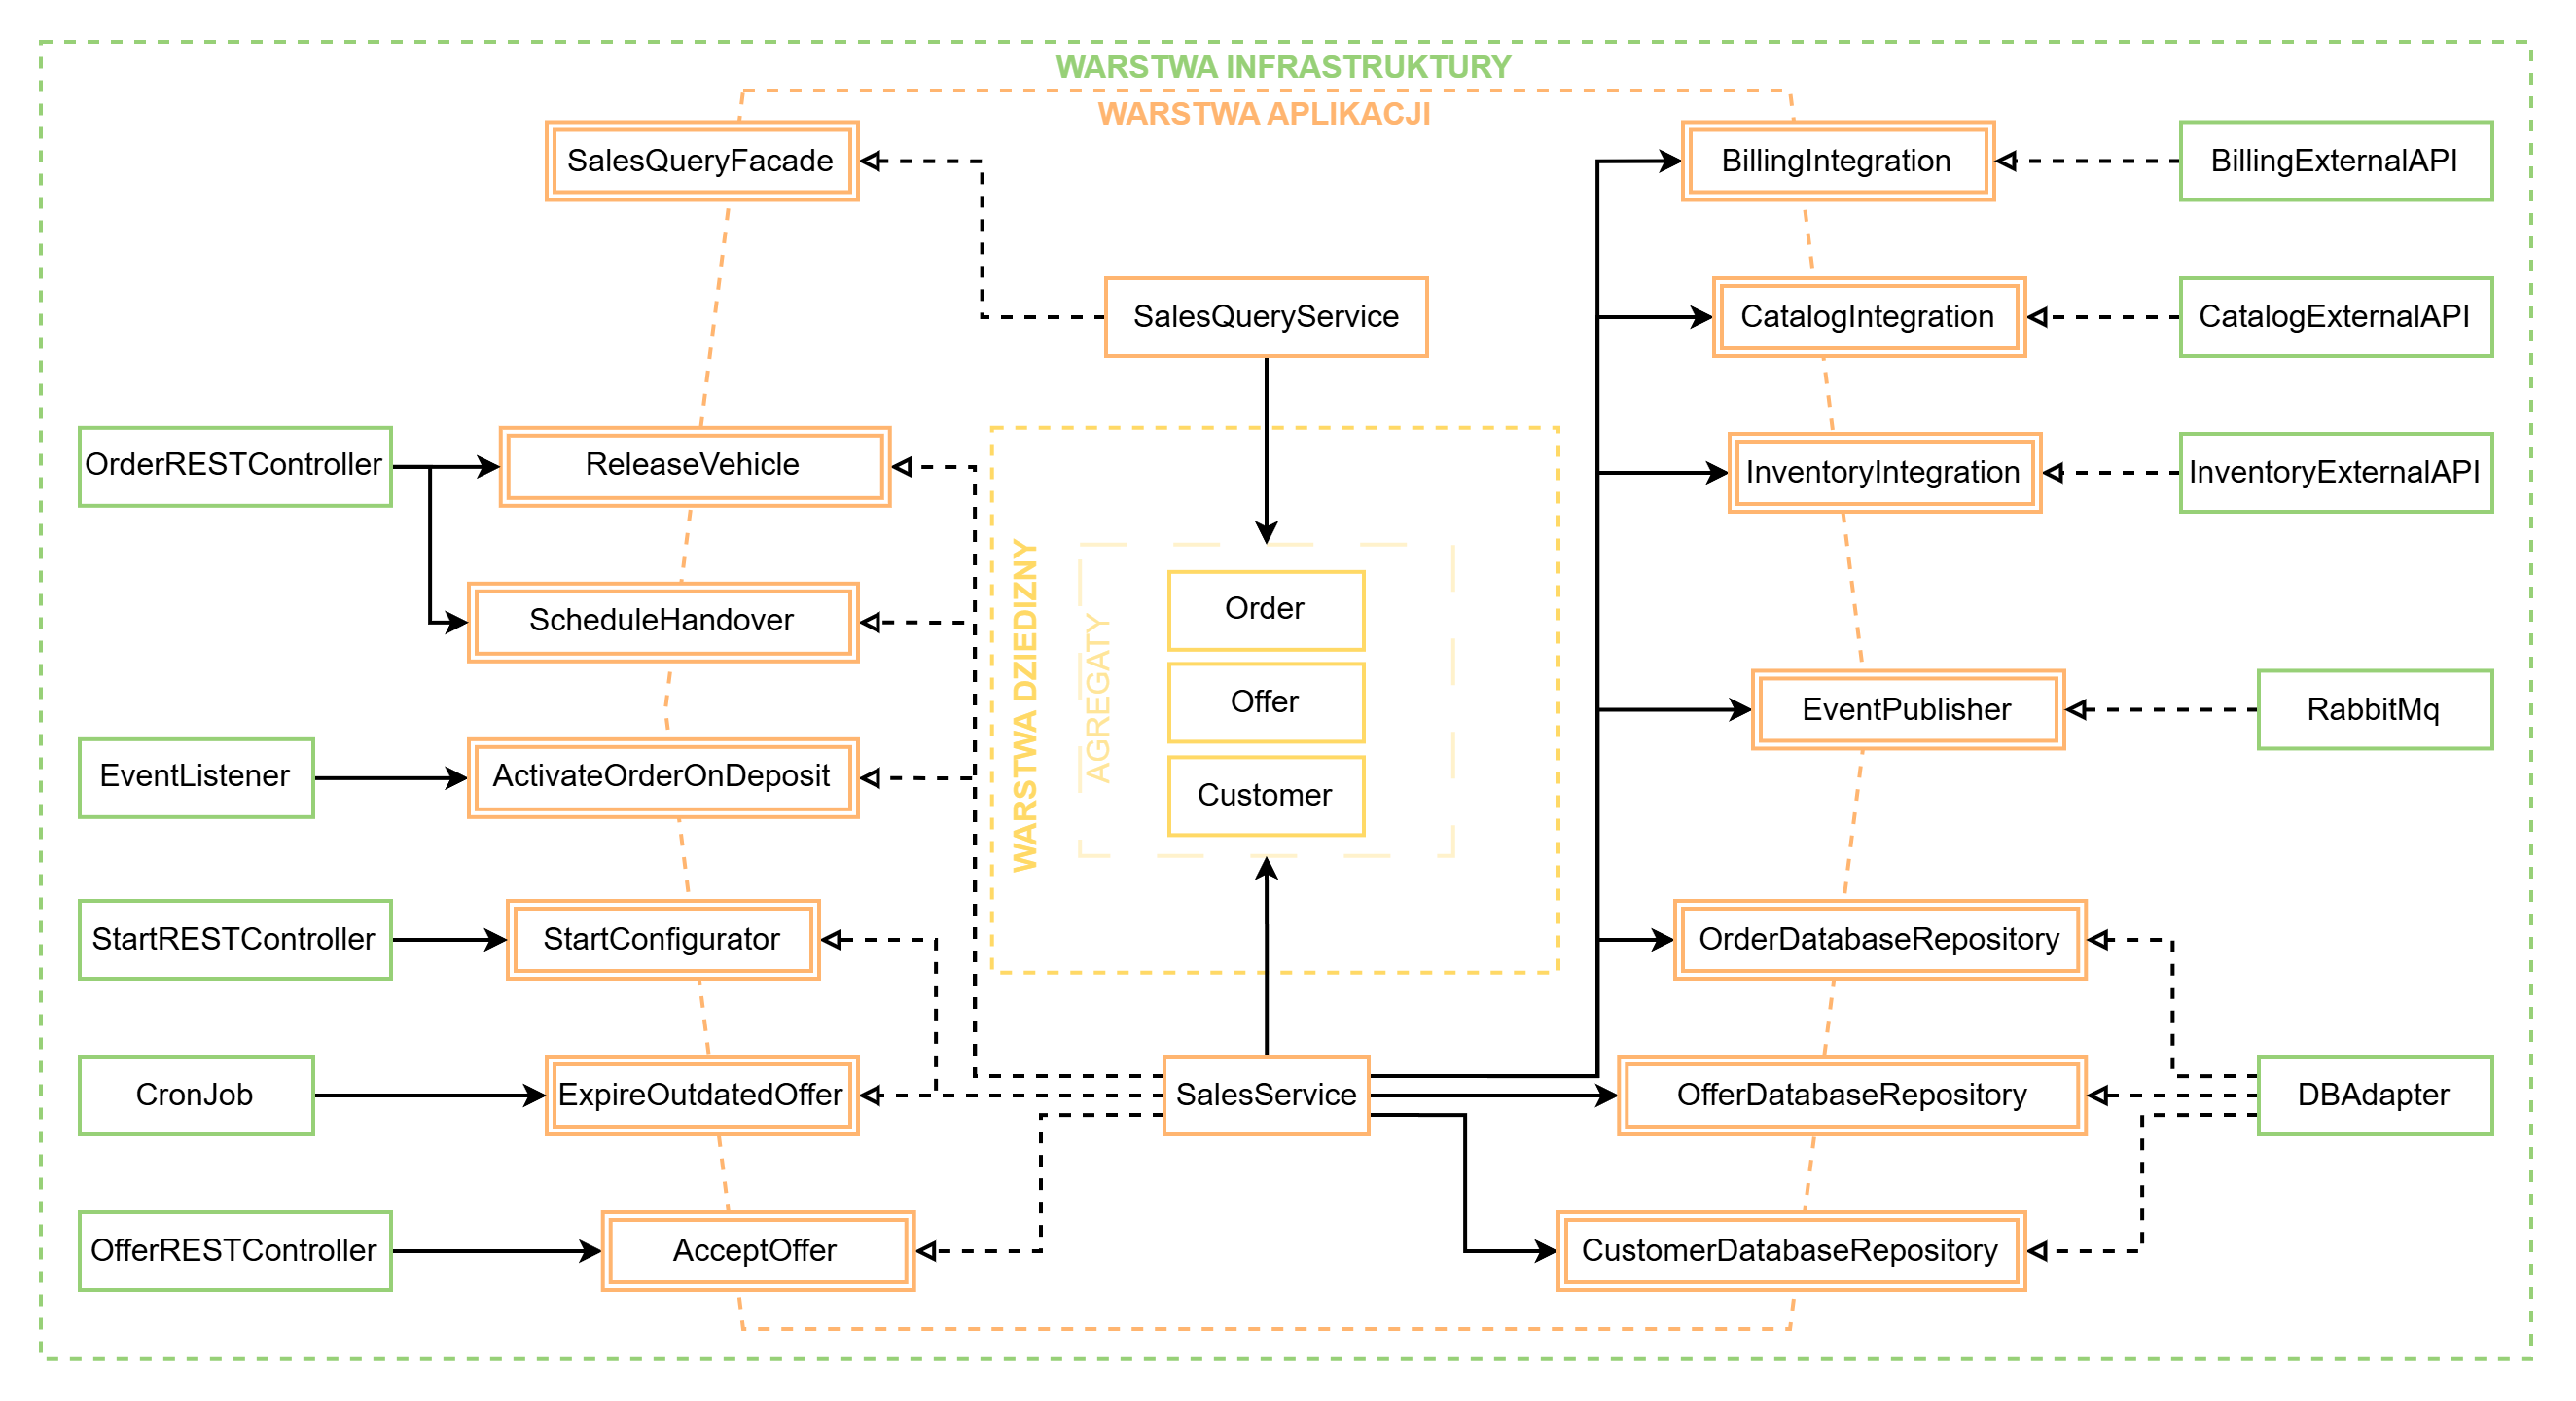
\includegraphics[width=\textwidth]{media/architektura_heksagonalna/SalesArchitecture.png}
    \caption{Architektura heksagonalna kontekstu sprzedaży i CRM}
    \label{fig:hex_sales}
\end{figure}

Poniżej przedstawiono szczegółowy opis interakcji pomiędzy warstwami, z podziałem na strony wejściową i wyjściową.

\paragraph{Strona Wejściowa: Porty i Adaptery} 
Ta strona heksagonu definiuje, w jaki sposób użytkownicy końcowi (klienci), handlowcy oraz inne moduły systemu inicjują procesy sprzedażowe.

\begin{itemize}
    \item \textbf{Inicjacja i Ofertowanie (Synchroniczne)}
    \begin{itemize}
        \item \textbf{Porty:} \texttt{StartConfigurator} (UC-CRM-01) oraz \texttt{ReceiveSpecificationUseCase} (UC-CRM-02). Interfejsy obsługujące bezstanowe otwarcie sesji konfiguratora oraz odbiór gotowej specyfikacji w celu wygenerowania wiążącej oferty.
        \item \textbf{Adaptery (HTTP):} \texttt{SessionRestApiAdapter} (sesje konfiguratora), \texttt{OfferRestApiAdapter} oraz \texttt{OrderRestApiAdapter}. Parsują żądania sieciowe z przeglądarki klienta na komendy domeny.
    \end{itemize}

    \item \textbf{Zarządzanie Transakcją i Wydaniem (Mieszane)}
    \begin{itemize}
        \item \textbf{Porty:} \texttt{AcceptOffer} (UC-CRM-03), \texttt{ActivateOrderOnDeposit} (aktywacja po wpłacie), \texttt{ScheduleHandover} (UC-CRM-04), \texttt{ReleaseVehicle} (UC-CRM-05) oraz \texttt{SynchronizeSpecificationPriceUseCase}. Interfejsy obsługujące konwersję oferty w zamówienie, koordynację wydań i zamknięcie procesu.
        \item \textbf{Adaptery:} Adaptery sieciowe (\texttt{OrderRestApiAdapter}, \texttt{InventoryWebhookRestAdapter}), adaptery nasłuchujące magistrali zdarzeń (\texttt{BillingEventSubscriberAdapter}, \texttt{CatalogEventSubscriberAdapter}, \texttt{LogisticsEventSubscriberAdapter}, \texttt{SalesDepositListener}) oraz \texttt{OfferExpirationCronJobAdapter} (cykliczne wygaszanie ofert). Adaptery zdarzeniowe reagują na sygnały z innych modułów (np. gotowość logistyczna z Inwentarza, zaksięgowanie wpłaty z Fakturowania), automatycznie wyzwalając odpowiednie porty.
    \end{itemize}
\end{itemize}

\paragraph{Strona Wyjściowa: Porty i Adaptery} 
Ta strona heksagonu definiuje zapotrzebowanie modułu Sprzedaży na utrwalanie wielowątkowego stanu biznesowego oraz komunikację z procesami logistyczno-finansowymi.

\begin{itemize}
    \item \textbf{Utrwalanie Stanu (Persystencja)}
    \begin{itemize}
        \item \textbf{Porty:} \texttt{CustomerDatabaseRepository}, \texttt{OfferDatabaseRepository} oraz \texttt{OrderDatabaseRepository}. Umożliwiają niezależny odczyt i zapis trzech głównych agregatów domeny.
        \item \textbf{Adaptery:} \texttt{OfferDatabaseAdapter} oraz \texttt{OrderDatabaseAdapter} — adaptery JPA (Hibernate; encje \texttt{OfferJpaEntity}/\texttt{OrderJpaEntity} i repozytoria Spring Data) z optymistyczną kontrolą współbieżności; \texttt{InMemoryCustomerRepository} — atrapa w pamięci dla klientów.
    \end{itemize}

    \item \textbf{Integracja Międzykontekstowa (Delegacja Zadań)}
    \begin{itemize}
        \item \textbf{Porty:} \texttt{InventoryIntegration}, \texttt{FinancingIntegrationPort}, \texttt{BillingIntegration}, \texttt{CatalogIntegration} oraz read-modele cen (\texttt{CatalogPriceQueryPort}, \texttt{SpecificationPriceReadModelPort}). Służą do koordynacji logistyki, finansowania i fakturowania oraz do lokalnego odczytu wyceny specyfikacji.
        \item \textbf{Adaptery:} \texttt{InventoryExternalApiAdapter}, \texttt{BillingExternalApiAdapter}, \texttt{CatalogExternalApiAdapter} (klienci HTTP z krótkim timeoutem), \texttt{FinancingEventBusAdapter} (zapytanie o zdolność przez publikację \texttt{FinancingRequestedEvent}), \texttt{InventoryCommandAdapter} oraz \texttt{InMemorySpecificationPriceReadModelAdapter}. Izolują jądro domeny od technicznych detali komunikacji z innymi kontekstami.
    \end{itemize}

    \item \textbf{Publikacja Zdarzeń}
    \begin{itemize}
        \item \textbf{Port:} \texttt{EventPublisher} (port Wspólnego Jądra). Interfejs zlecający emisję faktów biznesowych na zewnątrz modułu.
        \item \textbf{Adapter:} \texttt{SalesEventBusAdapter} (docelowo \texttt{RabbitMqEventPublisherAdapter} Wspólnego Jądra). Serializuje krytyczne zdarzenia dziedzinowe (np. \texttt{FinancingRequestedEvent}, \texttt{BankTransferDeclaredEvent}, \texttt{OrderPlacedEvent}) i umieszcza je na magistrali, umożliwiając modułom Fakturowania, Finansowania i Inwentarza asynchroniczną reakcję.
    \end{itemize}
\end{itemize}

\paragraph{Usługi Aplikacji}
W celu zapewnienia kontroli nad cyklem życia klienta zastosowano komplementarne komponenty koordynujące:
\begin{itemize}
    \item \textbf{SalesService} – główna usługa aplikacyjna orkiestrująca porty wejściowe sprzedaży (UC-CRM-02 do UC-CRM-05 oraz aktywacja po wpłacie). Pobiera agregaty (\texttt{Customer}, \texttt{Offer}, \texttt{Order}), wywołuje na nich dozwolone mutacje stanu, koordynuje porty integracyjne i utrwala wyniki w repozytoriach.
    \item \textbf{ConfiguratorAppService} – obsługa sesji konfiguratora (UC-CRM-01).
    \item \textbf{SalesQueryService} – realizacja publicznej fasady zapytań \texttt{SalesQueryFacade} (migawki nabywcy i oferty dla innych kontekstów).
\end{itemize}

\subsubsection{Agregaty Kontekstu Sprzedaży}

Cykl życia relacji handlowej został podzielony na dwa wyraźnie oddzielone od siebie etapy: niezobowiązujące negocjacje oraz prawnie wiążący kontrakt. Z uwagi na ich całkowicie odmienny cykl stanowy, zdekomponowano je na dwa niezależne agregaty.

% MIEJSCE NA DIAGRAM KLAS: Offer
\begin{figure}[h]
    \centering
    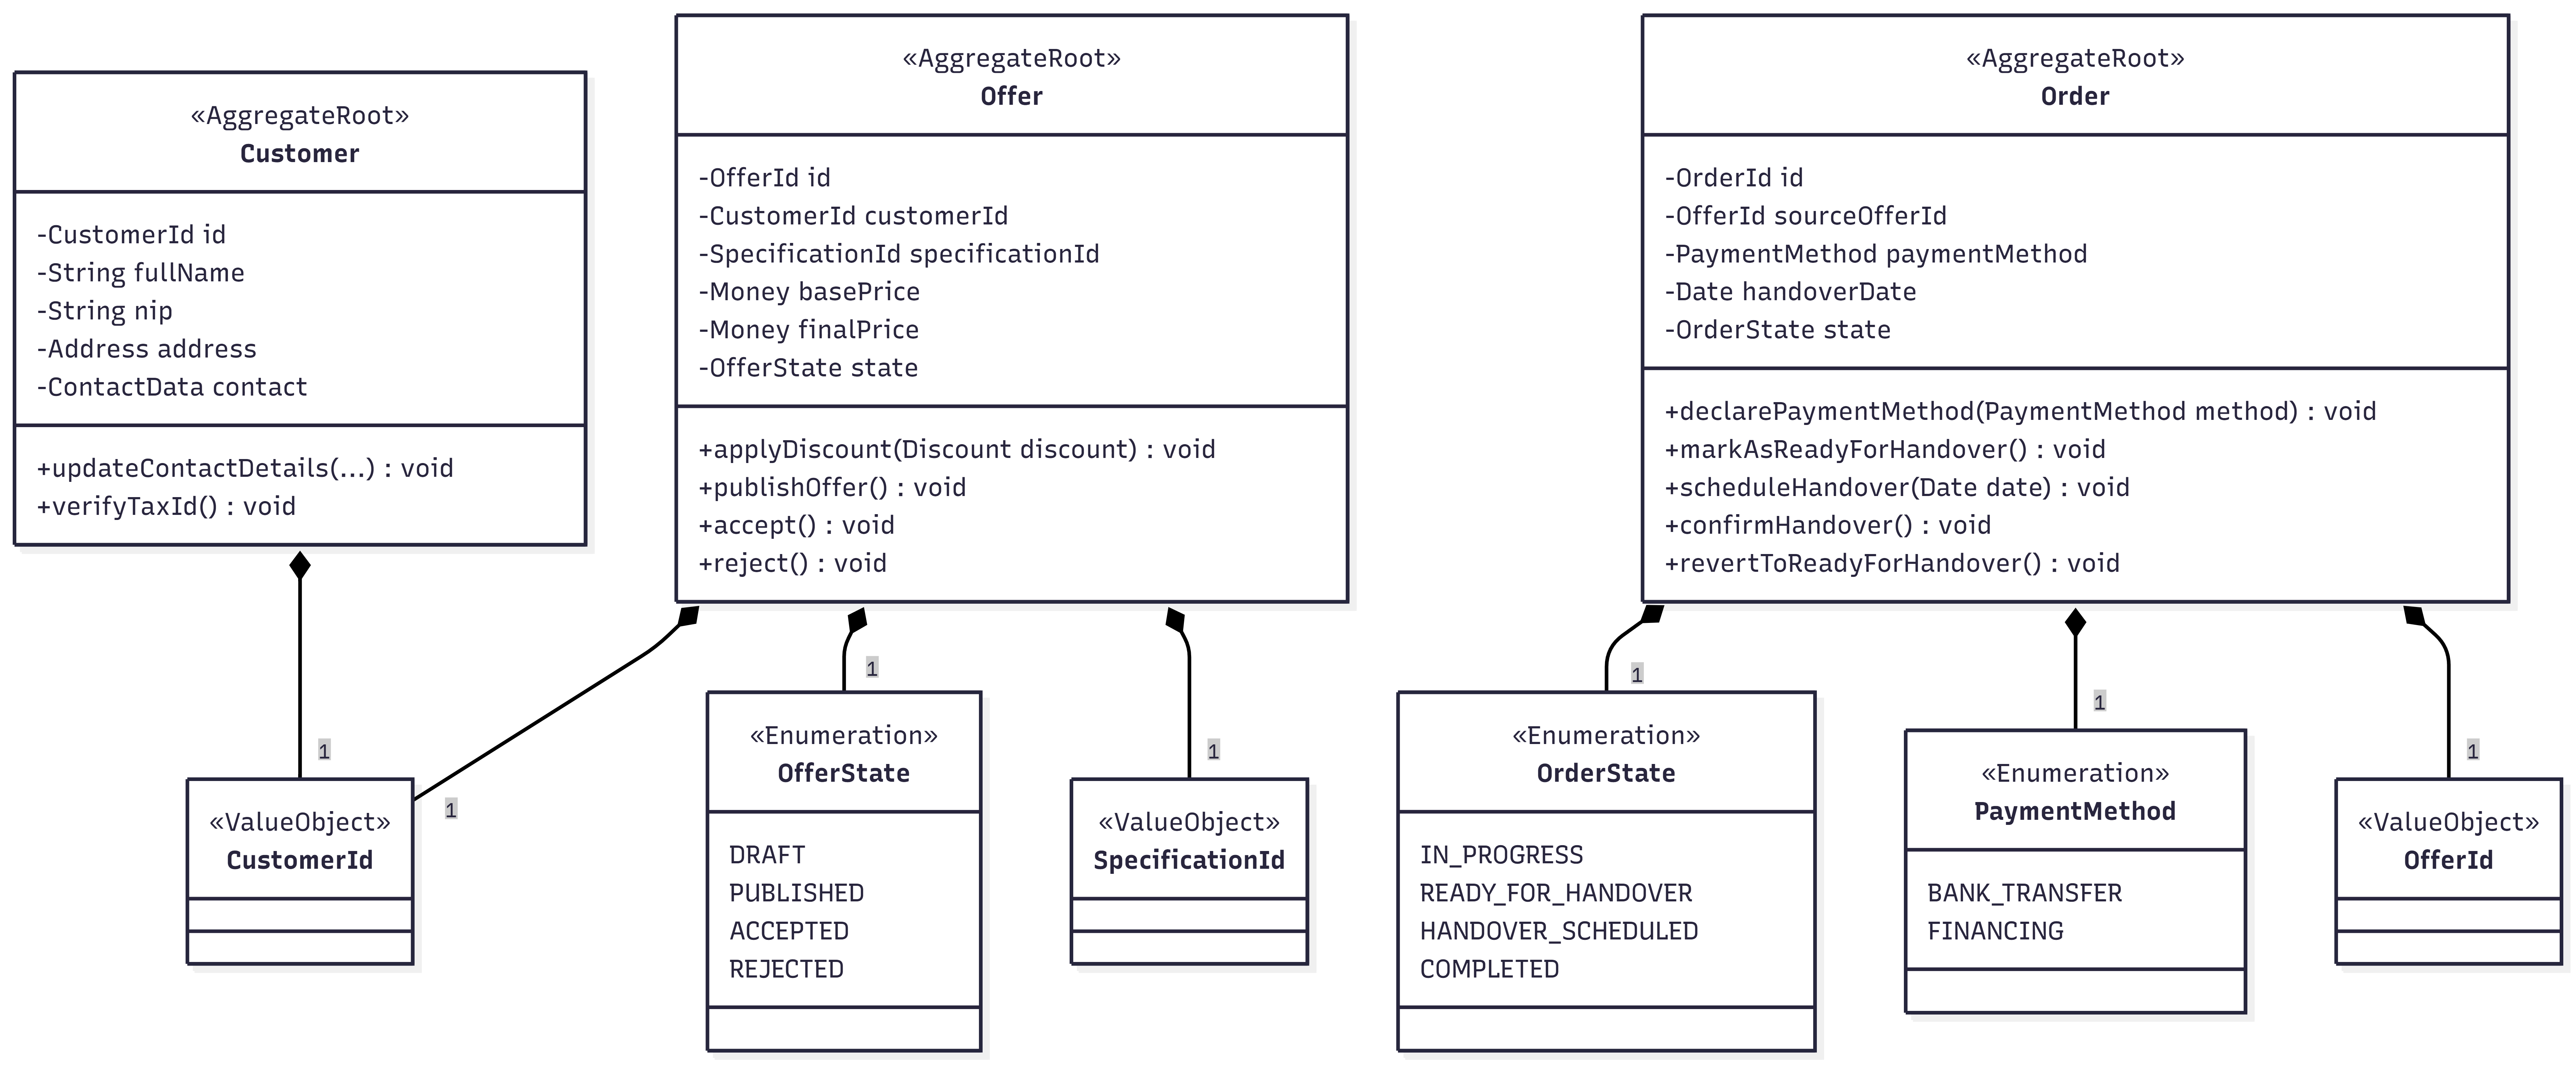
\includegraphics[width=\textwidth]{media/agregaty/kontekst-sprzedaży/customer-offer-order.png}
    \caption{Model strukturalny agregatu Oferty (Proforma).}
    \label{fig:agg_offer}
\end{figure}

Złożoność domeny CRM została opanowana poprzez ścisły podział odpowiedzialności pomiędzy trzy agregaty, które komunikują się ze sobą wyłącznie poprzez wzorzec referencji przez identyfikator.

\paragraph{Agregat: Klient (Customer)}
Stanowi rekord tożsamości klienta w systemie.
\begin{itemize}
    \item \textbf{Centralizacja Tożsamości:} Zamiast powielać dane osobowe w każdym dokumencie, agregat ten jest jedynym źródłem prawdy o kliencie. Pozostałe agregaty odwołują się do niego wyłącznie przez hermetyczny obiekt wartości \texttt{CustomerId}. Zapewnia to natychmiastową globalną spójność w przypadku np. zmiany adresu korespondencyjnego.
    \item \textbf{Weryfikacja Formalna:} Agregat zamyka w sobie logikę weryfikacyjną (np. \texttt{verifyTaxId()}), chroniąc system przed procesowaniem transakcji na podstawie błędnych danych podatkowych.
\end{itemize}

\paragraph{Agregat: Oferta (Offer)}
Tymczasowy byt biznesowy, zarządzający fazą negocjacji i kalkulacji rabatów.
\begin{itemize}
    \item \textbf{Hermetyzacja Decyzji Cenowych:} Metody mutujące, takie jak \texttt{applyDiscount()}, zamykają wewnątrz agregatu reguły ograniczające politykę rabatową. 
    \item \textbf{Maszyna Stanów:} Cykl życia oferty kończy się na jednoznacznym stanie terminalnym (\texttt{ACCEPTED} lub \texttt{REJECTED}). Po jego osiągnięciu agregat staje się całkowicie niemutowalny, pełniąc rolę historycznego dowodu wynegocjowanych warunków.
\end{itemize}

\paragraph{Agregat: Zamówienie (Order)}
Realizuje logistyczną, finansową i fizyczną część procesu wydania pojazdu.
\begin{itemize}
    \item \textbf{Polityka Płatności i Logistyki:} Agregat przechowuje stan wykonawczy \texttt{OrderState} oraz zarządza kluczowymi deklaracjami (np. \texttt{declarePaymentMethod()}). Metody cyklu życia, takie jak \texttt{scheduleHandover()} oraz \texttt{confirmHandover()}, hermetyzują reguły gotowości pojazdu do wydania fizycznego.
    \item \textbf{Mechanizmy Kompensacyjne (Saga):} W systemach rozproszonych mogą wystąpić awarie na styku kontekstów (np. niepowodzenie wyksięgowania pojazdu z Inwentarza podczas fizycznego wydania). Agregat \texttt{Order} obsługuje takie przypadki dzięki jawnej metodzie kompensacyjnej \linebreak \texttt{revertToReadyForHandover()}, co zapewnia ostateczną spójność i bezpieczny powrót do poprzedniego stabilnego stanu.
\end{itemize}